\chapter{Introduction}
\section{Background and research purpose}
In the foreseeable future, the electrification of ocean systems, renewable ocean power sources, and ocean energy networks will be necessary, which will help accelerate the growth and deployment of ocean renewable energy and ways to explore and understand the ocean \cite{Orekan, Randhawa2015}. To achieve electrification in the ocean, it is necessary to deploy corresponding sensor networks underwater and process the data received by underwater sensors in a timely manner (Figure \ref{fig:underwater sensor networks}). At the same time, underwater sensors are also an essential tool for studying the marine environment \cite{Heidemann2012, Wu2020}. They can easily and flexibly explore underwater terrain and ecological environment, which provides convenience for the deployment of underwater sensor networks. An excellent AUV needs to have good equipment waterproofness, long-distance underwater controllability, and power durability. For the water-resistance of the equipment, we can use high-performance waterproof and pressure-resistant materials \cite{Hwang2019, Tran2020}. The remote controllability needs to solve the problems of long-distance underwater wireless communication. The durability of electrical equipment requires low energy consumption AUV and high-energy batteries or a continuous power supply. Sufficient power supply can keep underwater sensors and AUVs in an efficient and stable working state for a long time \cite{Jurdak2006}. Indirectly, reducing human interference when electrical equipment is working underwater can also improve work efficiency and reduce deployment costs. Therefore, the energy supply for underwater electrical equipment has become a novel research direction. Such methods can solve the energy supply problem of underwater equipment economically and ensure the system to perform long-term and stable work [3].

\begin{figure}[htbp]
    \centering
    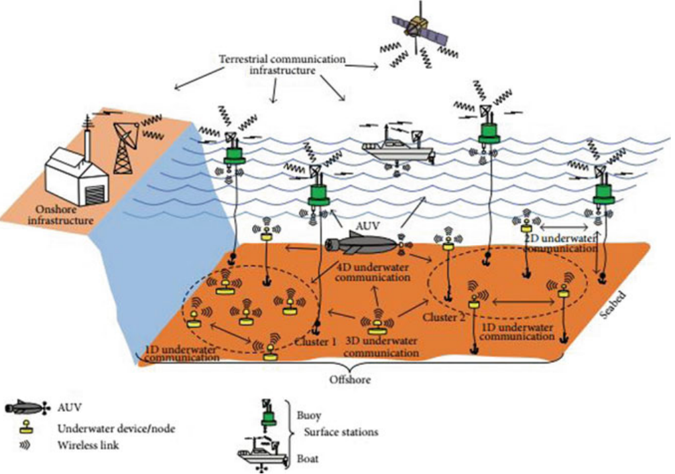
\includegraphics[width=0.7\linewidth]{images/1_underwater_sensor_networks.png}
    \caption{Underwater sensor networks architecture \cite{Nayyar}.}
    \label{fig:underwater sensor networks}
\end{figure}

In traditional marine engineering, power is supplied to underwater equipment through wet-mate subsea connectors [4]. For the traditional wet plug interface technology, its high cost, complex docking method, poor safety performance, and easy to be corroded by seawater, make its disadvantages in marine engineering increasingly obvious. Wireless Power Transfer (WPT) simplifies the connection between underwater equipment and power supply, reduces the continuous operating cost of underwater equipment, saves a lot of resources, and gradually gains the favor of scholars.

The ocean itself and its surroundings contain a lot of energy, such as tidal energy, wave energy, marine current power, ocean thermal energy, and sea salinity gradient power \cite{Capareda2019, Drew2009, Vlachogiannis2014, Zeng2020}. Ocean energy is rich, widely distributed, clean, and pollution-free, but low energy density and strong regionality. These advantages make it attractive as grid-connected energy, and may also make it an isolated and remote ocean energy source, thereby providing a valuable source of ocean space. Continuous development provides power solutions that are attractive. The rapid development of distributed ocean energy applications (such as underwater sensor networks, ocean sensors and monitoring technologies, ocean automatic network buoys, and deep-sea and tsunami buoys) is beneficial. In particular, it can power an autonomous underwater vehicle (AUV) whose service life is limited by its battery power.


\section{Wireless power transfer technologies}

Broadly speaking, power transfer without direct electrical contact between the primary and secondary is wireless power transfer. Wireless power technology can be divided into two main categories, near-field (nonradiative region) power transfer and far-field (radiative region) power transfer. 
Near-field means the area within about 1 wavelength ($\lambda$) of the antenna. The range of near-field devices is conventionally divided into two categories [ref] (Suppose the distance between two antennas is represented by $D_{range}$, and the diameter of two antenna coils is represented by $D_{ant}$.):
\begin{itemize}
    \item  Short range, the distance between two antennas is less than the diameter of antenna: $D_{range} \leq D_{ant}$. In this range, power is usually transferred through non-resonant capacitive or inductive coupling.
    \item Mid-range, the distance between two antennas is less than 10 times the diameter of antenna:  $D_{range} \leq 10 D_{ant}$. In this range, energy is usually transferred through resonant capacitive or inductive coupling.
\end{itemize} 

\begin{table}[!t]
    \centering
    \caption{The different wireless power transmission technologies.}
    \resizebox*{\textwidth}{!}{
    \begin{tabular}{ |c|c|c|m{3.5cm}<{\centering}|m{3.5cm}<{\centering}| }
        % \thickhline
        \hline
        \textbf{Technology} & \textbf{Range} & \textbf{Frequency}         & \textbf{Antenna devices}                    & \textbf{Applications}                             \\\hline
        % \thickhline
Microwaves          & hm – km        & GHz                        & Parabolic dishes, phased arrays, rectennas  & Satellite, drone aircraft                         \\ \hline
Optical             & dam – km
                    & $\geq$THz      & Lasers, photocells, lenses & Drone aircraft, space elevator                                                                  \\ \hline
Capacitive          & cm – m         & kHz – MHz                  & Metal plate electrodes                      & Smartcards, biomedical implant
\\ \hline
Inductive           & mm – m         & Hz – GHz                   & Tuned wire coils, lumped element resonators & Electric toothbrush, smartphone, electric vehicle
\\ \hline
    \end{tabular}
    }
    \label{table:differentWPT}
\end{table}


\begin{figure}[!b]
    \resizebox*{\textwidth}{!}{
    \begin{subfigure}{0.5\textwidth}
        \centering
        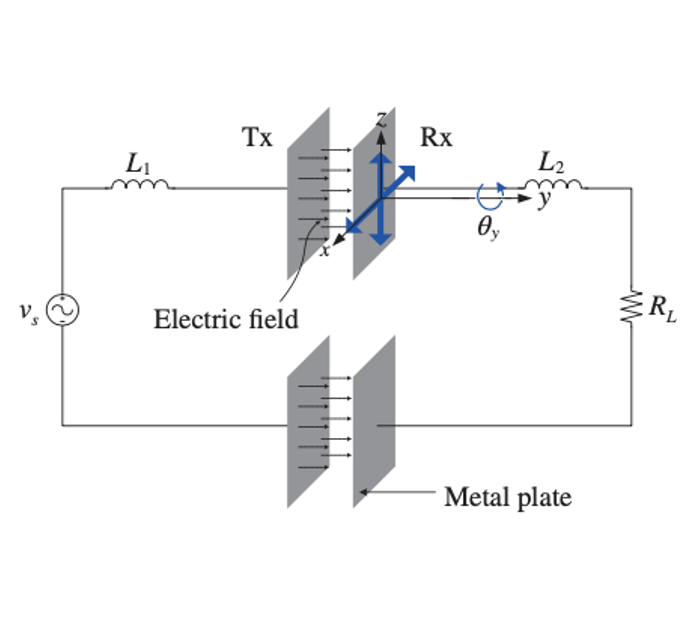
\includegraphics[width=0.9\linewidth]{images/1_capacitive_power_transfer.png}
        \caption{Capacitive power transfer \cite{Chun}.}
        \label{fig:subim1}
    \end{subfigure}
    \begin{subfigure}{0.5\textwidth}
        \centering
        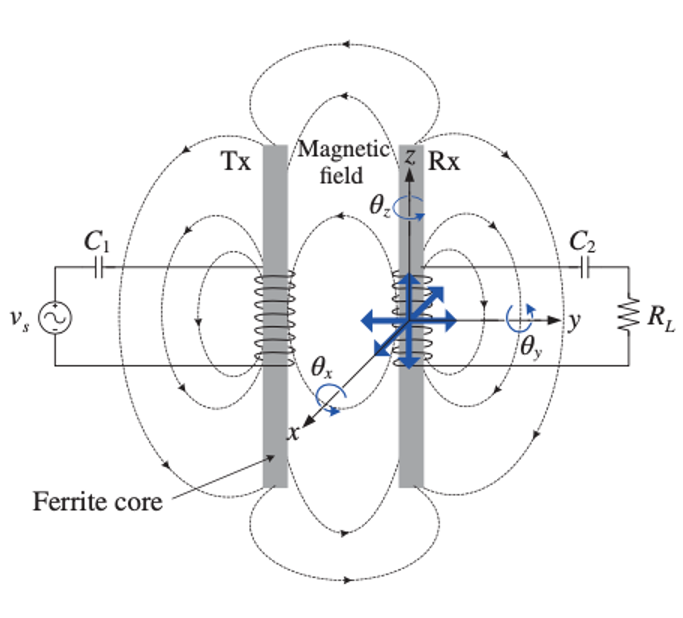
\includegraphics[width=0.9\linewidth]{images/1_inductive_power_transfer.png}
        \caption{Inductive power transfer \cite{Chun}.}
        \label{fig:subim2}
    \end{subfigure}}

    \caption{Near-field wireless power transfer.}
    \label{fig:near-fieldwpt}
\end{figure}


\begin{figure}[!t]
    \resizebox*{\textwidth}{!}{
    \begin{subfigure}{0.5\textwidth}
        \centering
        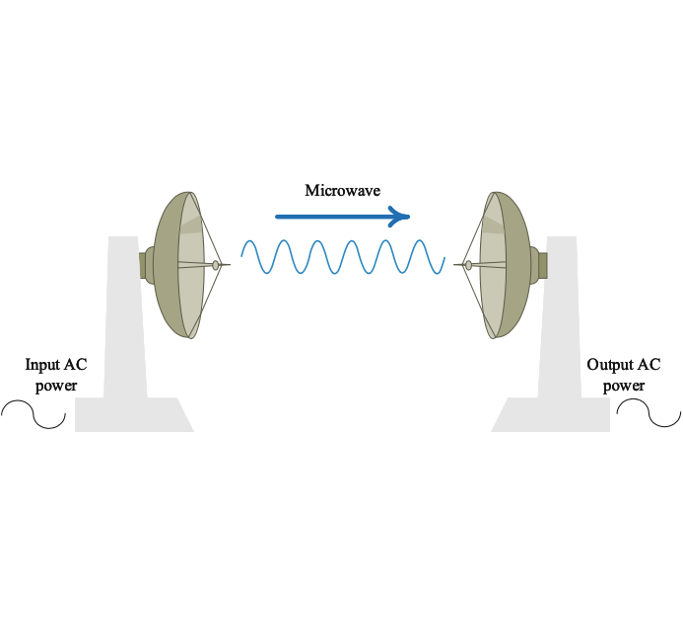
\includegraphics[width=0.9\linewidth]{images/1_microwave_power_transfer.png}
        \caption{Microwave power transfer \cite{Orekan}.}
        \label{fig:subim1}
    \end{subfigure}
    \begin{subfigure}{0.5\textwidth}
        \centering
        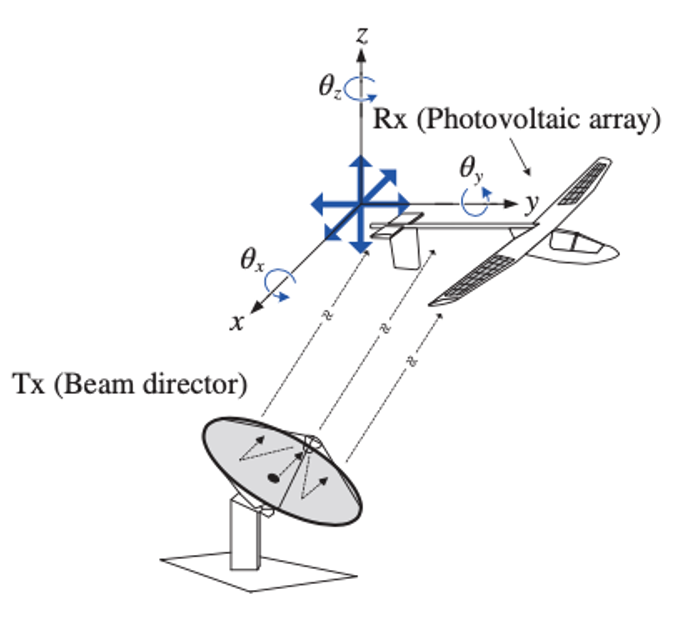
\includegraphics[width=0.9\linewidth]{images/1_laser_power_transfer.png}
        \caption{Laser power transfer \cite{Chun}.}
        \label{fig:subim2}
    \end{subfigure}
    }
    \caption{Far-field wireless power transfer.}
    \label{fig:far-fieldwpt}
\end{figure}


Far-field or radiative region, power is transmitted by means of electromagnetic waves, like radio waves, microwaves, or light waves. When the operating frequency ($f$) is relatively low, wavelength $\lambda = c/f$, at this time the diameter of the antenna is much smaller than the wavelength, $D_{ant} \ll \lambda$, and the radiated power will be very small. When the diameter of antenna is about wavelength, $D_{ant} \approx \lambda$, radiate power will be efficient. When the diameter of antenna is much great than wavelength, $D_{ant} \gg \lambda$, we can using high-gain antennas to concentrate electromagnetic waves on a narrow beam and directly aim at the receiver to improve transmission efficiency.


Therefore, near-field wireless power transfer systems mainly include inductive coupling power transfer and capacitive coupling power transfer (Figure \ref{fig:near-fieldwpt}). Far-field wireless power transfer systems mainly include microwave, optical, and acoustic power transfer (Figure \ref{fig:far-fieldwpt}).  The respective characteristics are shown in the table \ref{table:differentWPT}.


\section{Underwater wireless power transfer}
WPT technology has unique advantages in special environments, and along with the continuous development of landing application research and the emergence of a large number of results, it has attracted the attention of underwater technology researchers. 
\subsection{Underwater environment}
In the seawater environment, we usually need to consider the following points.

\begin{itemize}
    \item Underwater, seawater has a blocking effect on high-frequency electromagnetic waves. The distance of electromagnetic waves propagating underwater is inversely proportional to the frequency, making it difficult to achieve long-distance power transmission.
    \item Conductivity, due to the electrical conductivity of seawater, traditional wireless power transmission analysis methods are no longer applicable. At present, the system modeling and related theoretical analysis of underwater wireless power transfer technology need to be improved.
    \item Undercurrent, the submarine landform is complex and there is undercurrent. The coupler core is liable to drift under water, and there are problems such as difficulty in docking, which results in low transmission efficiency.
    \item Some other impects, like microbial enrichment, temperature, salinity, etc.
    
\end{itemize}

\subsection{Common UWPT systems}

\begin{figure}[!t]
    \centering
    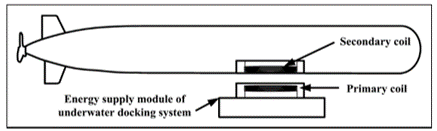
\includegraphics[width=0.7\linewidth]{images/1_stacked_UWPT_system.png}
    \caption{Stacked UWPT system \cite{Song}.}
    \label{fig:stacked UWPT system}
\end{figure}
Figure \ref{fig:stacked UWPT system} shows a stacked UWPT system, this study was completed by Baowei Song et al \cite{Song}. They achieved a transmission efficiency of 72\% while maintaining 100w output power.
They are using a saddle structure transmitter (Details as shown in figure \ref{fig:stacked UWPT system detail}) and a deformed cylindrical receiver. This structure is very convenient for AUT to park, but because there is no stable protection structure, it is also easy to shift when charging.

\begin{figure}[!t]
    \centering
    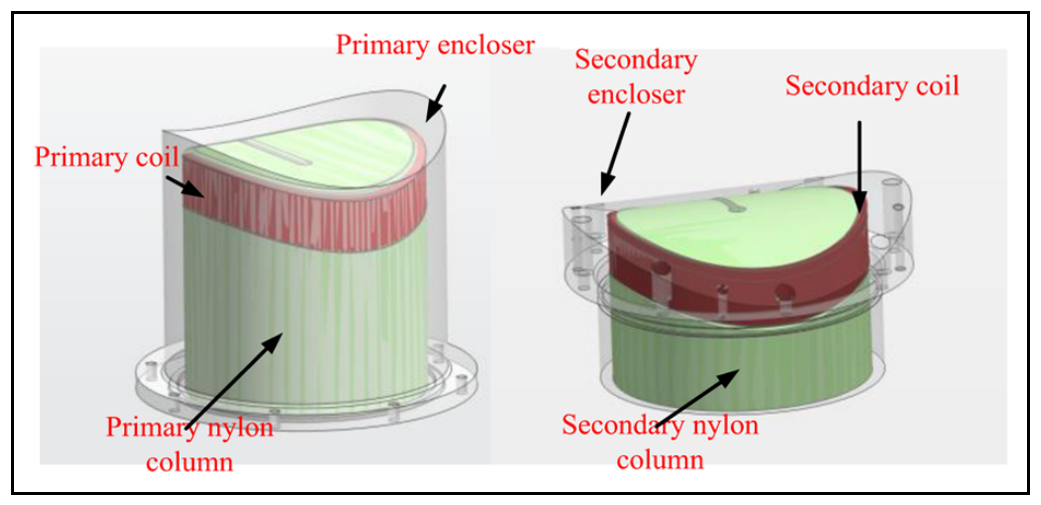
\includegraphics[width=0.7\linewidth]{images/1_stacked_UWPT_system_details.png}
    \caption{The primary and secondary coils of stacked UWPT system \cite{Song}.}
    \label{fig:stacked UWPT system detail}
\end{figure}

Figure \ref{fig:plug in UWPT system} shows the plug-in UPWT system. We can observe that the AUV needs to be moved into a hollow cylindrical structure transmitter, which makes it difficult to park. However, this structure can maintain the stability of the AUV during AUV charging, so that the system charging is more secure. Another advantage of this structure is that the receiving coil is relatively large, which can make the mutual inductance high. And we can use this system to transmit larger power. Therefore, our coil-array structure UWPT system is built on this structure.
\begin{figure}[!t]
    \centering
    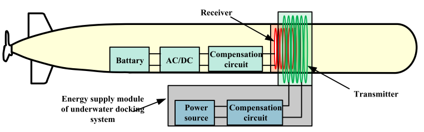
\includegraphics[width=0.7\linewidth]{images/1_plugin_UWPT_system.png}
    % \caption{Plug-in UWPT system [wang].}
    \caption{Plug-in UWPT system \cite{Wang2019}.}
    \label{fig:plug in UWPT system}
\end{figure}


\section{The main research content of this thesis}
This paper mainly studies the underwater wireless power transfer system, and analyzes the difference between the underwater environment and the land environment WPT system. Considering the durability and high reliability of underwater AUV, this paper proposes a novel coil array power transfer system. 
It provides reference materials for the subsequent research on the wpt system of multiple coil groups.

\section{Roadmap}
The first chapter analyzes the background of this research and its research purpose and significance, analyzes the characteristics and advantages and disadvantages of mainstream WPT technology, and provides a basis for using IPT technology as an underwater wireless energy transmission system in the following text. A detailed summary and analysis of the current research status of related technologies at home and abroad, including underwater wired energy transmission technology, WPT technology in underwater and air media, and an explanation of the research focus of this article.

The second chapter focuses on the analysis of the basic theory of wireless energy transmission. First, the basic IPT model is explained, and its working principle is analyzed. Then explained the related technology of compensation network. Finally, analyze the underwater IPT system model.

% 第三章初步探究了水下环境对场景wpt系统的影响。首先,通过测量三种不同介质中的Z-paremeter来观察不同介质中wpt系统参数的变化情况。然后再通过改变内部线圈的大小从而改变线圈间距离,来判断不同距离下wpt系统参数的变化。最后通过改变不同的工作频率,来观察不同评论下系统的参数变化情况。
The third chapter initially explores the influence of the underwater environment on the scene wpt system. First, by measuring the Z-paremeter in three different media to observe the changes of the wpt system parameters in different media. Then by changing the size of the internal coil to change the distance between the coils, to judge the change of the wpt system parameters at different distances. Finally, by changing different working frequencies, we can observe the changes of system parameters under different comments.

% Chapter 3 first analyzes the basic principle of the parallel MRC-WPT circuit, and then based on the WPT model of the ordinary air-core coil, respectively, to address the horizontal offset and angular offset of the transmitter coil and the receiver coil, a new type of battery that can meet the charging requirements is proposed. The wireless energy transmission method of two-dimensional air-core coil and three-dimensional air-core coil enables the transmission efficiency of the underwater MRC-WPT system to be steadily improved. According to the structural characteristics of each method, the corresponding underwater wireless robot model is designed to meet the application conditions.
% 第四章介绍了我们提出的coil-array线圈结构。通过Wipl-d软件进行模拟,比较了coil-array线圈结构与two-ring结构的磁场分布与系统传输效率。然后通过实验,比较了几种不同coil-array arrangements的表现。总结出不同arrangements的优劣。
Chapter four introduces the coil-array coil structure we proposed. The simulation was carried out by Wipl-d software, and the magnetic field distribution and system transmission efficiency of the coil-array coil structure and the two-ring structure were compared. Then through experiments, we compared the performance of several different coil-array arrangements. Summarize the pros and cons of different arrangements.
% The fourth chapter first studies the magnetic field characteristics of the air gap coil, focusing on the analysis of the magnetic core's restraining effect on the coil magnetic field, and simulates the magnetic field distribution of the coil containing the air gap core, and proposes a new type of four-phase core coil. The method of wireless energy transmission. By studying the transmitting phase of the four transmitting coils, the induced magnetic fields in the four receiving coils will not cancel each other, and stable energy transmission can be carried out. Then the four-phase magnetic core coil transmission scheme is simulated. Aiming at the characteristics of its magnetic field distribution, the AUV model proposed in the previous article is taken as an example, and a universal application model of the structure is designed under water.

% 第五章总结了前文中的实验结果和一些不足。并针对这些不足提出了一些能将实验表现提高的建议,这些内容写在了未来工作里面。
Chapter five summarizes the experimental results and some shortcomings in the previous article. In response to these shortcomings, some suggestions that can improve the performance of the experiment are put forward, which are written in the future work.